\documentclass{beamer}
\usetheme{Warsaw}

\usecolortheme[rgb={0,0.57,0.92}]{structure}
\definecolor{grayColor}{rgb}{0.255,0.25,0.275}
\setbeamercolor{section in head/foot}{bg=grayColor,fg=white}
\setbeamerfont{subsection in head/foot}{size=\tiny}

\setbeamerfont{section in toc}{size=\small}
\setbeamerfont{subsection in toc}{size=\scriptsize}

\usepackage[T1]{fontenc}
\usepackage[utf8]{inputenc}
\setbeamertemplate{footline}[frame number]{}
\setbeamertemplate{navigation symbols}{}


\title{Expériences sur les nombres premiers}
\author{Aymeric BEAUCHAMP\\Dimitri CHAGNEUX\\Valentin LEBLOND\\Baptiste MORI}
\date{18 Mars 2019}

\begin{document}
\maketitle
\section*{}
\subsection*{Sommaire}
\frame{\tableofcontents}

\section{Notre projet}

\subsection{Nombre premier}%Aymeric%
\begin{frame}
\begin{block}{Définition}
Un nombre premier est un entier naturel qui admet exactement deux diviseurs distincts : 1 et lui-même.
\end{block}
\begin{itemize}
\item Traces de leur découverte dès l'Antiquité (Euclide)
\item Énormément de propriétés liées à leur répartition, aux tests de primalité, etc.
\end{itemize}
$\Rightarrow$ Un des objets mathématiques les plus connus 
\end{frame}

\subsection{Applications en informatique}%Aymeric%
\begin{frame}
\structure{Cryptographie à clé publique (RSA)}
\begin{itemize}
\item Une clé privée pour lire les messages : deux nombres premiers \textit{x} et \textit{y}
\item Une clé publique pour envoyer les messages : le produit $x*y$
\end{itemize}
Factorisation d'un entier en facteurs premiers : problème considéré NP-complet\\
\vspace{0.5cm}
\structure{Autres applications}\\
\vspace{0.25cm}
Tables de hachage, générateurs aléatoires...
\end{frame}

\subsection{Objectifs}
\begin{frame}
\begin{itemize}
\item 
\item 
\item 
\item 
\end{itemize}
\end{frame}

\section{Détection des nombres premiers}
\subsection{Crible d'Eratosthène}
\begin{frame}

\end{frame}

\subsection{Petit théorème de Fermat}

\begin{frame}
\structure{Présentation}
\begin{itemize}
\item énoncé pour la première fois en 1640
\item nombreuses applications
\end{itemize}
\end{frame}

\begin{frame}
\structure{Dans notre cas}
\begin{itemize}
\item[] test de primalité
\item[] 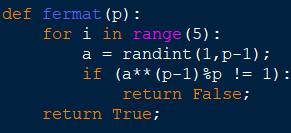
\includegraphics[scale=1]{images/fermat_code.png}
\end{itemize}
\end{frame}

\begin{frame}
\structure{Résultats}
\begin{itemize}
\item avec 733\\ 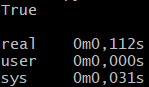
\includegraphics[scale=1]{images/fermat1.png}
\item avec 3 000 000\\ 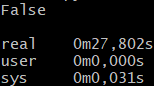
\includegraphics[scale=1]{images/fermat4.png}
\item avec 9 999 991\\ 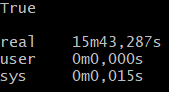
\includegraphics[scale=1]{images/fermat5.png}
\end{itemize}
\end{frame}

\subsection{Exponentiation modulaire}
\begin{frame}
\structure{Présentation}
\begin{itemize}
\item permet une élévation à la puissance modulo un entier
\item calcul naïf
\item méthode directe
\end{itemize}
\end{frame}

\begin{frame}
\structure{Dans notre cas}
\begin{itemize}
\item[] 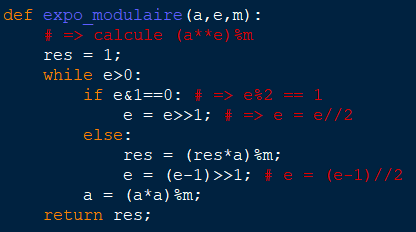
\includegraphics[scale=1]{images/expo_mod.png}
\end{itemize}
\end{frame}

\begin{frame}
\begin{block}{Utilisation avec le test de primalité de Fermat}
on remplace le test dans notre test de primalité par un appel à la fonction d'exponentiation modulaire
\end{block}
\end{frame}

\begin{frame}
\begin{itemize}
\item 733\\ 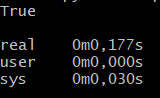
\includegraphics[scale=0.7]{images/expo1.png}
\item 3 000 000\\ 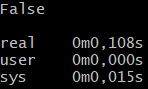
\includegraphics[scale=0.7]{images/expo4.png}
\item 9 999 991\\ 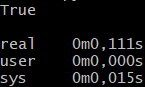
\includegraphics[scale=0.7]{images/expo5.png}
\item liste des nombres premiers entre 3 et 1 000 000\\
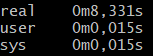
\includegraphics[scale=0.9]{images/expo_1000000.png}
\end{itemize}
\end{frame}

\subsection{Génération de polynômes}
\begin{frame}

\end{frame}

\section{Nombres de Mersenne}
\subsection*{Présentation}
\begin{frame}
\begin{block}{Définition}
Les nombres de Mersenne sont les nombres qui s'expriment sous la forme :
\begin{center}
$M_{n} = 2^{n}-1, n\geq1$
\end{center}
\end{block}
$\Rightarrow$ Sous-suite des nombres premiers de Mersenne\\
\vspace{0.25cm}
Ils sont les plus grands nombres premiers connus à ce jour\\
\vspace{0.25cm}
Record actuel : $M_{82 589 933}$, découvert en décembre 2018
\end{frame}

\subsection{Recherche dans un fichier}
\begin{frame}
\begin{itemize}
\item Utilisation d'un fichier contenant 300 millions de nombres premiers
\item Le plus grand nombre de Mersenne contenu dans le fichier est $M_{31}=2 147 483 647$
\item Tous les nombres de Mersenne premiers du fichier trouvés en deux heures
\end{itemize}
\end{frame}

\subsection{Test de Lucas-Lehmer}
\begin{frame}
Soit une suite \textit{s} définie de la manière suivante :
$$
    \begin{array}{ll}
        s_{0} = 4 \\
        s_{i+1} = s_{i}^{2}-2 \\
    \end{array}
$$
Pour $p>2$, $M_{p}$ est premier si et seulement si $s_{p-2}$ \textit{mod} $M_{p} = 0$.\\
\begin{itemize}
\item Pour comparer avec la précédente méthode, on fait les tests jusqu'à $M_{31}$.\\
\item Temps total : 1 heure et 9 secondes
\end{itemize}
\end{frame}

\begin{frame}
\begin{center}
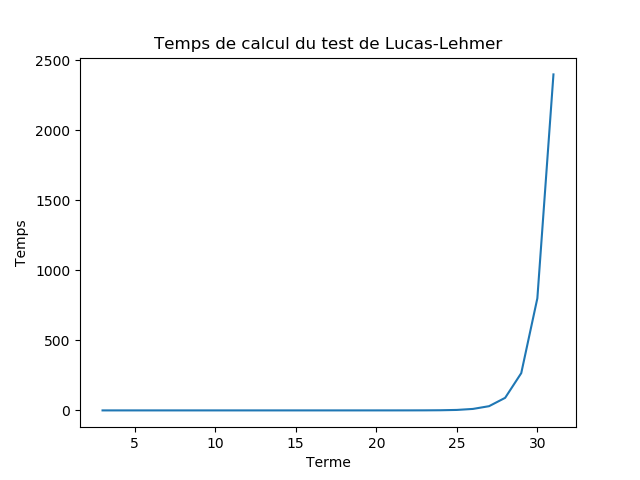
\includegraphics[scale=0.5]{images/evo_lucas.png}
\end{center}
\end{frame}

\section{Spirale d'Ulam}
\subsection*{Présentation}
\begin{frame}
\begin{center}
\vspace{-1cm}
Spirale d'Ulam
\end{center}
\begin{center}
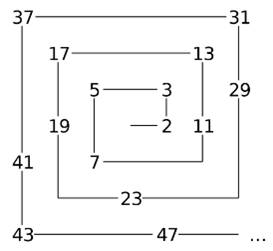
\includegraphics[scale=0.7]{images/spirale_explication.jpg}
\hspace{0.5cm}

\includegraphics[scale=0.25]{images/spirale_explication.PNG}
\end{center}
\end{frame}

\subsection{Réalisation}
\begin{frame}
\begin{itemize}
\item Utilisation d'un curseur afin de remplir la grille en spirale
\item Java avec Swing pour l'interface graphique
\end{itemize}
\vspace{0.5cm}
\begin{center}
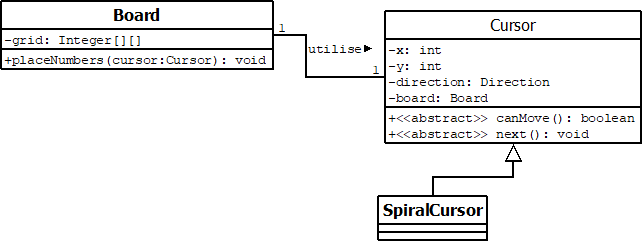
\includegraphics[scale=0.45]{images/dia_spirale.png}
\end{center}
\end{frame}

\begin{frame}
\begin{center}
\vspace{0.5cm}

\includegraphics[scale=0.5]{images/s1.PNG}
\end{center}
\end{frame}

\begin{frame}
\begin{center}
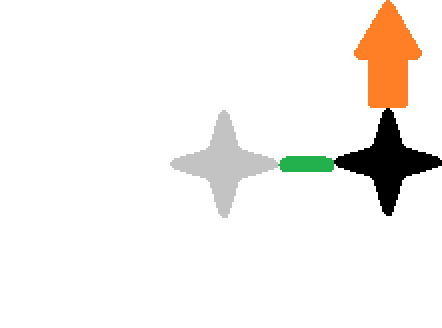
\includegraphics[scale=0.5]{images/s2.PNG}
\end{center}
\end{frame}

\begin{frame}
\begin{center}
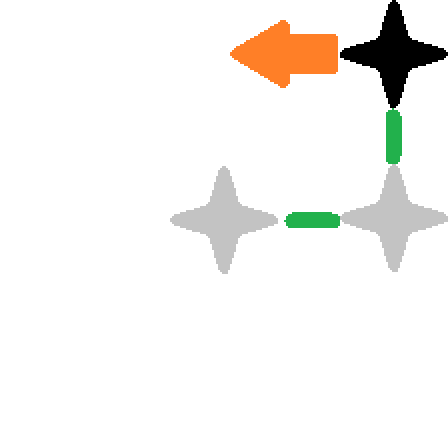
\includegraphics[scale=0.5]{images/s3.PNG}
\end{center}
\end{frame}

\begin{frame}
\begin{center}
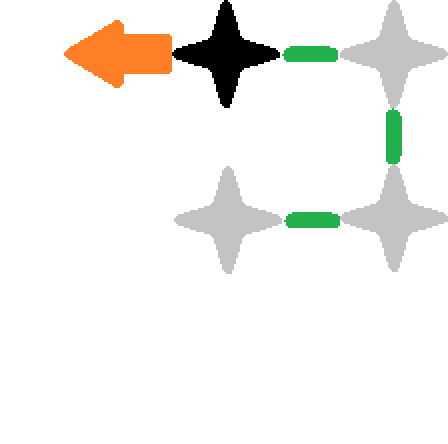
\includegraphics[scale=0.5]{images/s4.PNG}
\end{center}
\end{frame}

\begin{frame}
\begin{center}
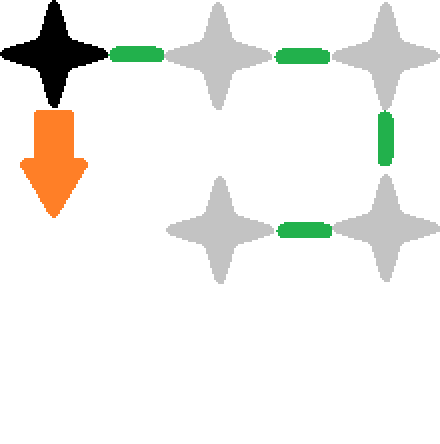
\includegraphics[scale=0.5]{images/s5.PNG}
\end{center}
\end{frame}

\begin{frame}
\begin{center}
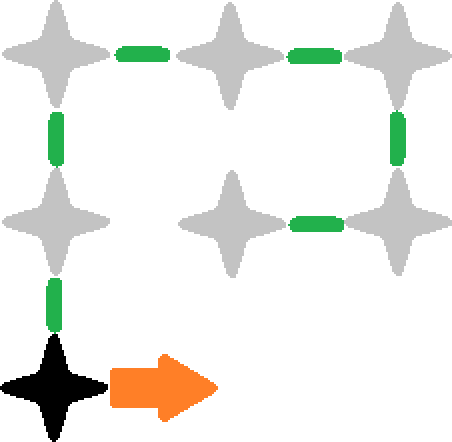
\includegraphics[scale=0.5]{images/s6.PNG}
\end{center}
\end{frame}

\begin{frame}
\begin{center}
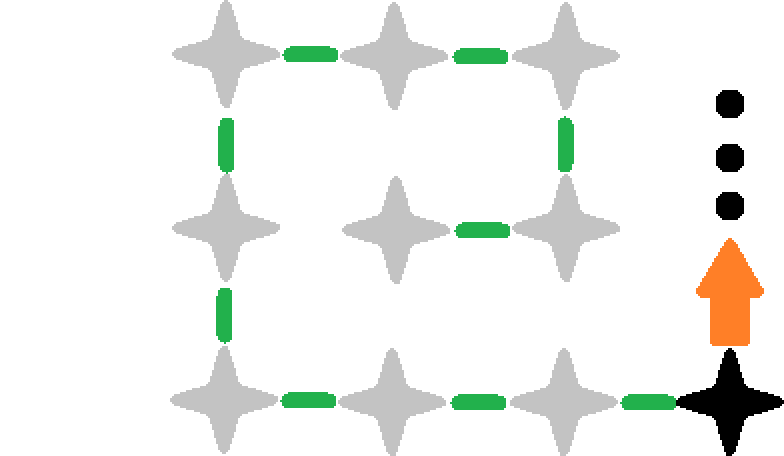
\includegraphics[scale=0.5]{images/s7.PNG}
\end{center}
\end{frame}

\begin{frame}
\begin{center}
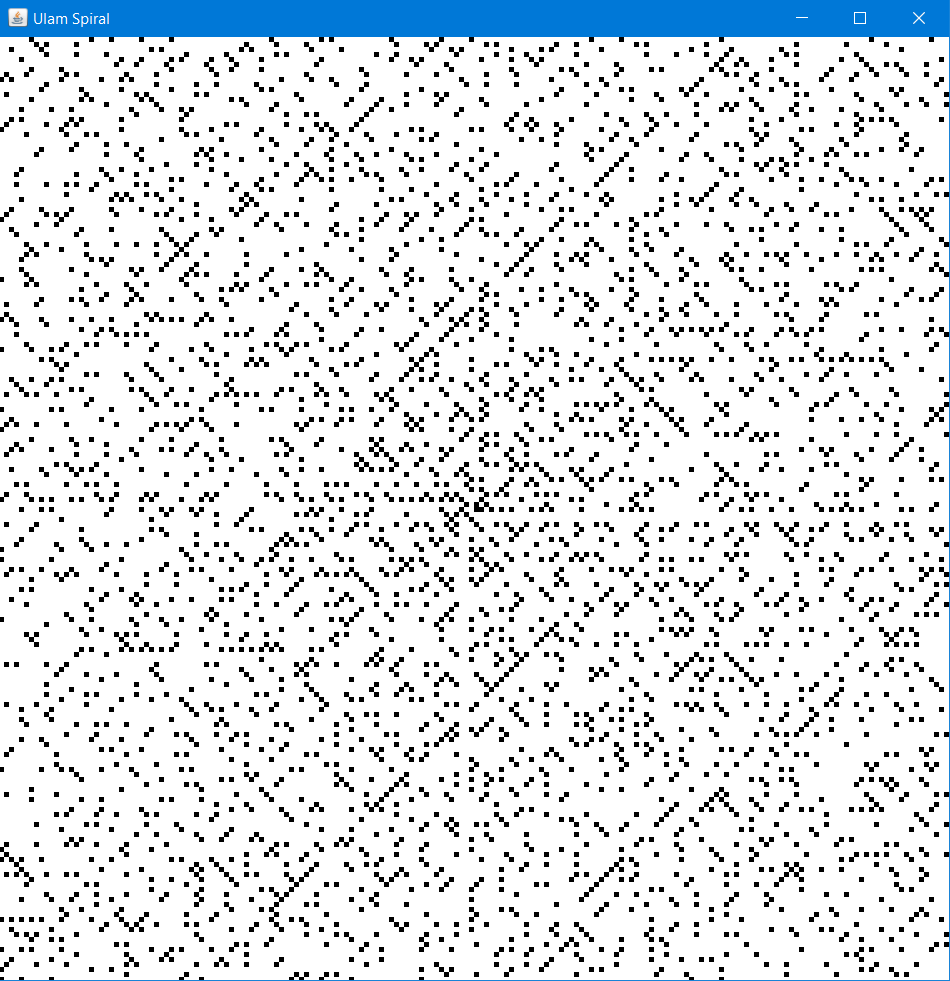
\includegraphics[scale=0.35]{images/spirale_1.PNG}
\end{center}
\end{frame}

\subsection{Observations}
\begin{frame}
\begin{center}
Nombre de départ : 41\\
\vspace{0.1cm}
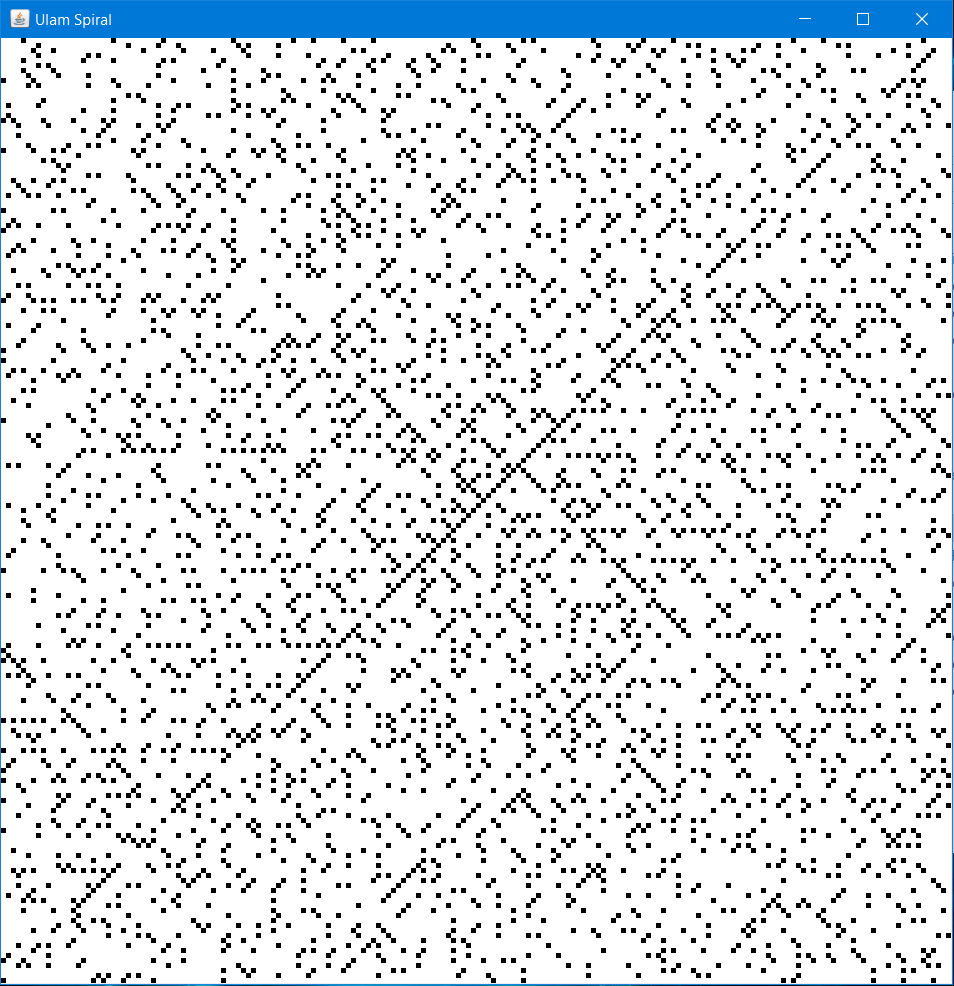
\includegraphics[scale=0.3]{images/spirale_41.PNG}
\end{center}
\end{frame}

\begin{frame}
\begin{center}
Nombre de départ : 104\\
\vspace{0.1cm}
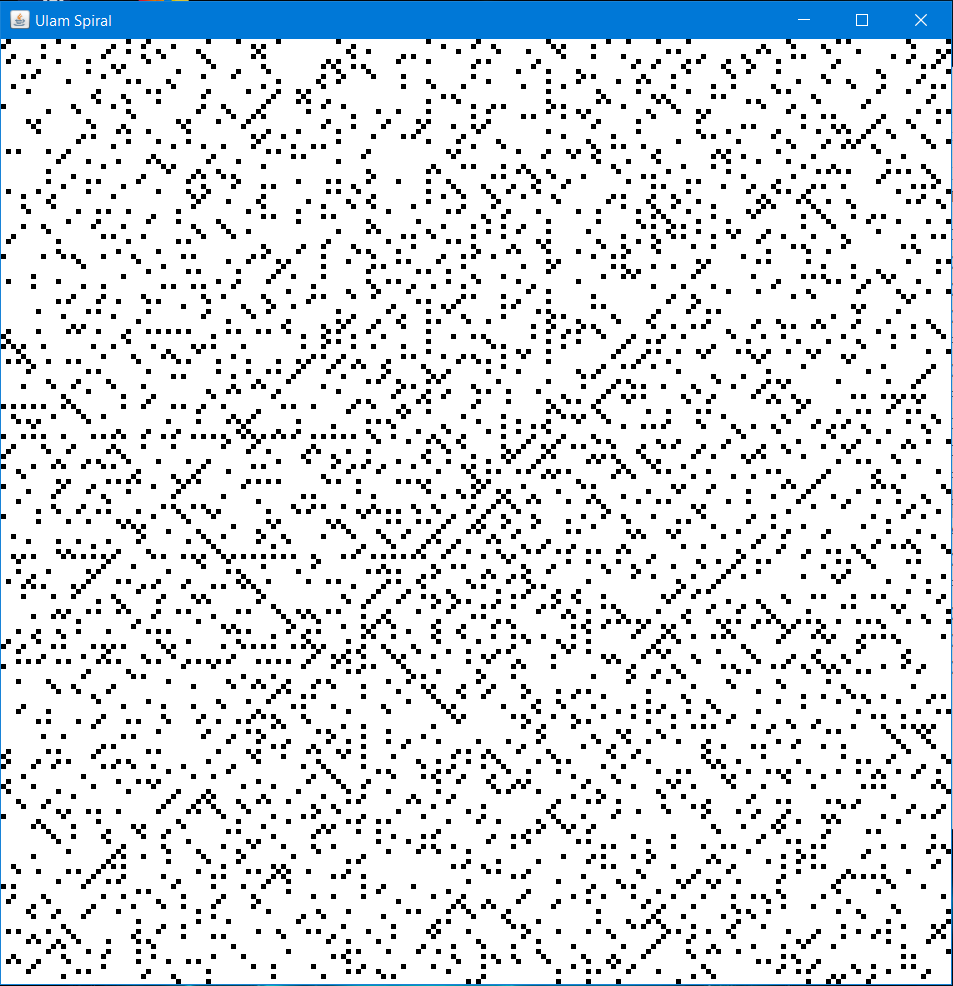
\includegraphics[scale=0.3]{images/spirale_104.PNG}
\end{center}
\end{frame}

\begin{frame}
\begin{center}
Nombre de départ : 1 et 1548468615\\
\vspace{0.2cm}
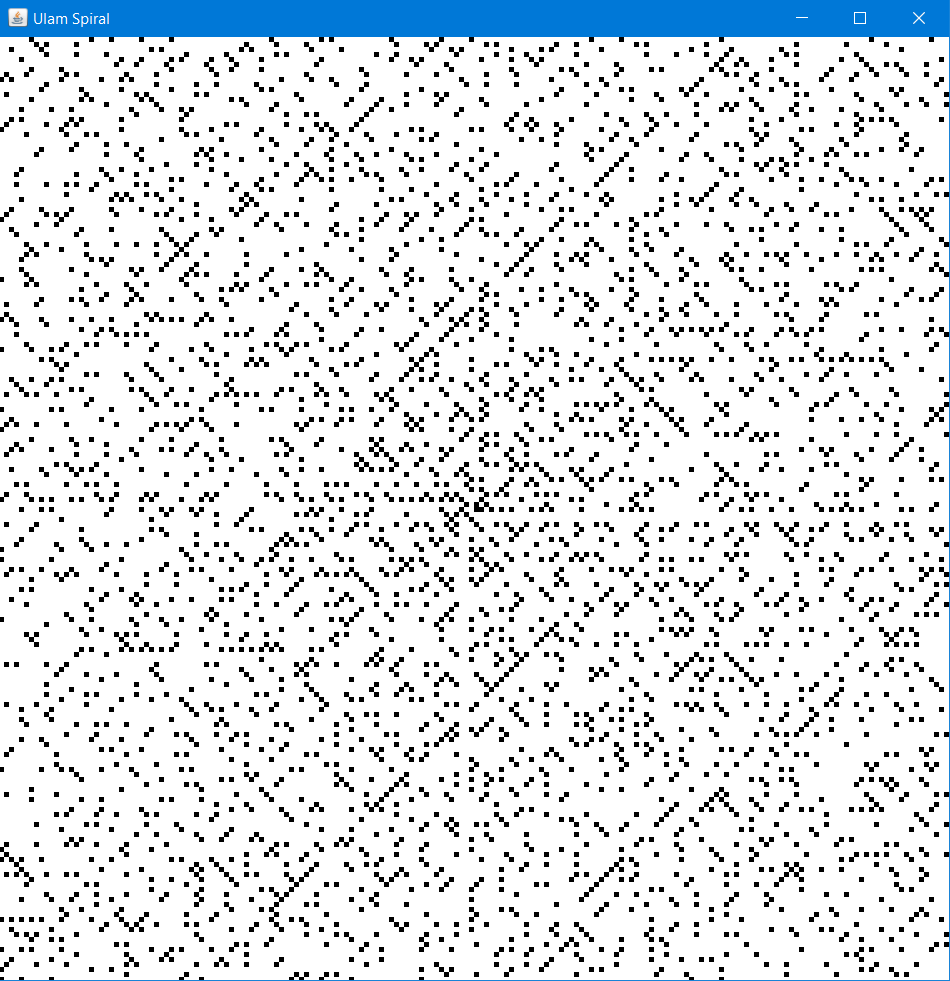
\includegraphics[scale=0.25]{images/spirale_1.PNG}
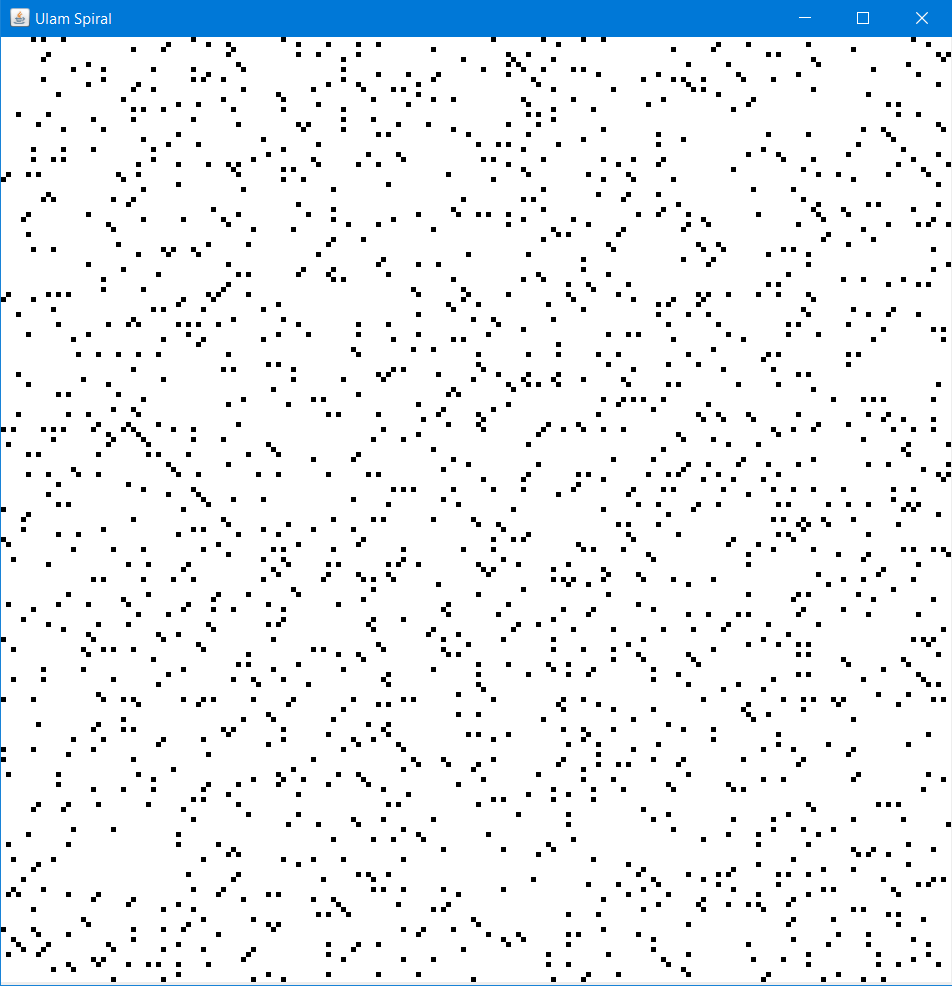
\includegraphics[scale=0.25]{images/spirale_grandNB.PNG}
\end{center}
\end{frame}

\section{Syracuse (3n+1)}
\subsection*{Présentation}
\begin{frame}
\begin{block}{Définition}
La suite de Syracuse s'exécute sur un nombre donné k, on divise ce nombre par 2 si k est pair, ou on le multiplie par 3 et ajoute 1 si celui-ci est impair ; on réitère jusqu'à ce qu'on obtienne 1. \\
\vspace{0.4cm}
On a donc une suite $(U_n)$ avec $U_0 = k$ et 
$$
U_{n+1} = \left\{
    \begin{array}{ll}
        U_n/2 & \mbox{si } U_n \mbox{ pair} \\
        3*U_n + 1 & \mbox{si } U_n \mbox{ impair} \\
        1 \mbox{ fin} & \mbox{si } U_n = 1
    \end{array}
\right.
$$
\vspace{0.1cm}
\end{block}
Exemple sur 3 :
$$
U_0 = 3, U_1 = 10, U_2 = 5, U_3 = 16, U_4 = 8, U_5 = 4, U_6 = 2, U_7 = 1, fin.
$$

\end{frame}

\subsection{Réalisation}
\begin{frame}
\begin{itemize}
\item Java en Swing
\item graphique en bar sur le nombre d'itérations
\item graphique des variations lors de l'exécution de la suite
\end{itemize}
\end{frame}

\begin{frame}
Graphique en bar de 2 à 100 :
\begin{center}
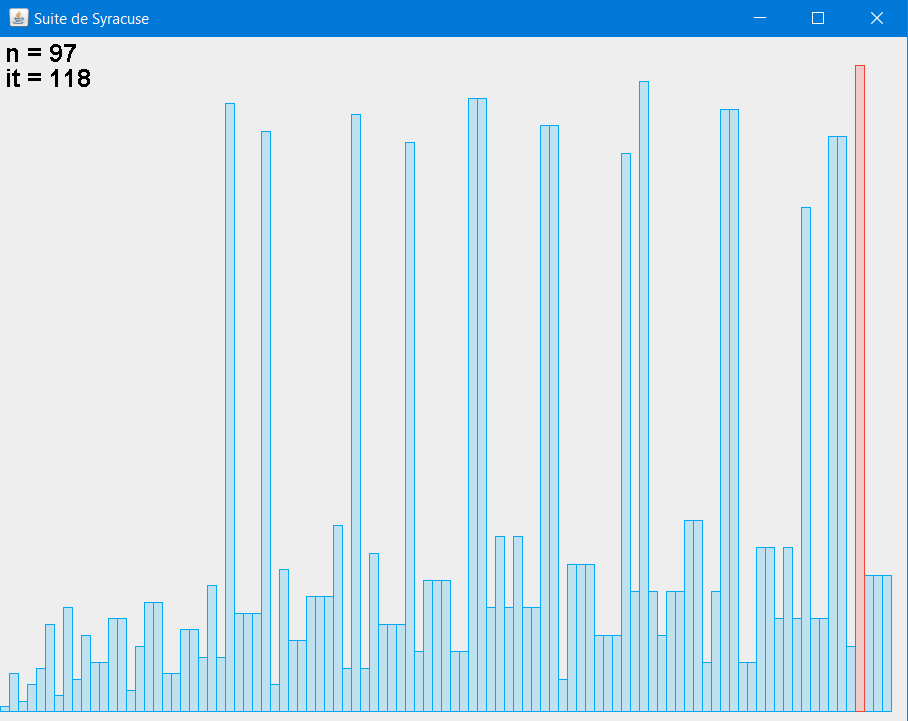
\includegraphics[scale=0.45]{images/syracuse_100.PNG}
\end{center}
\end{frame}

\begin{frame}
Variations avec 97 :
\begin{center}
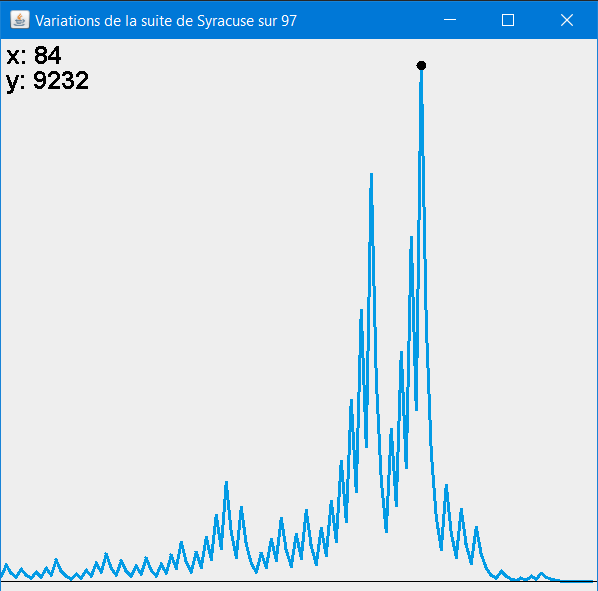
\includegraphics[scale=0.55]{images/syracuse_var_97.PNG}
\end{center}
\end{frame}

\subsection{Observations}
\begin{frame}
Séries de nombres consécutifs avec même nombre d'itérations :
\begin{center}
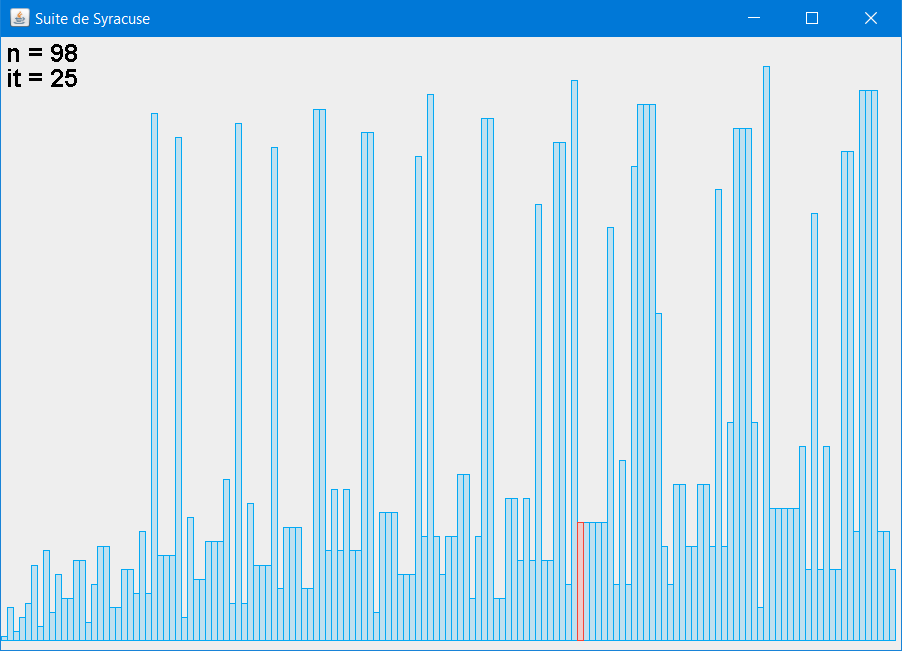
\includegraphics[scale=0.5]{images/syracuse_150.PNG}
\end{center}
\end{frame}

\begin{frame}
Même fin de variations pour certains nombres :
\begin{center}
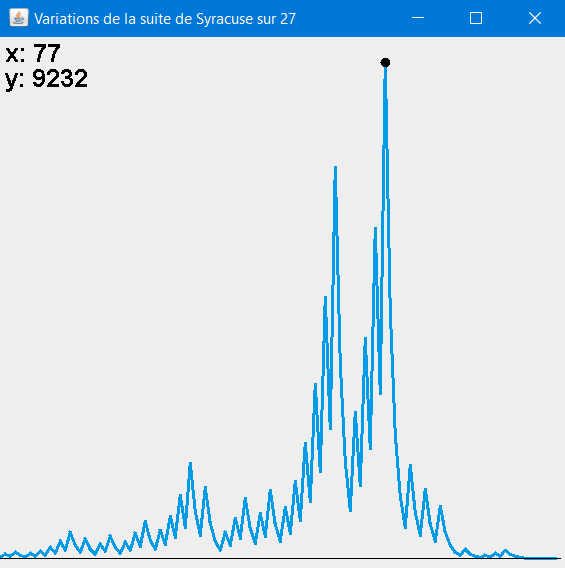
\includegraphics[scale=0.43]{images/syracuse_var_27.PNG}
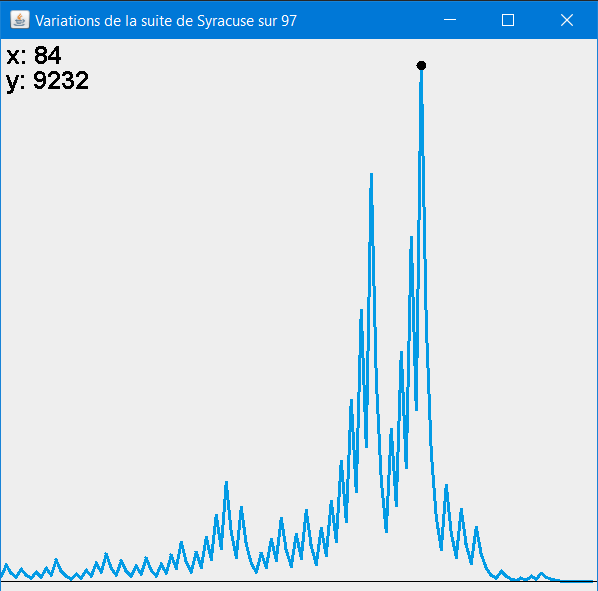
\includegraphics[scale=0.41]{images/syracuse_var_97.PNG}
\end{center}
\end{frame}

\begin{frame}
\begin{center}
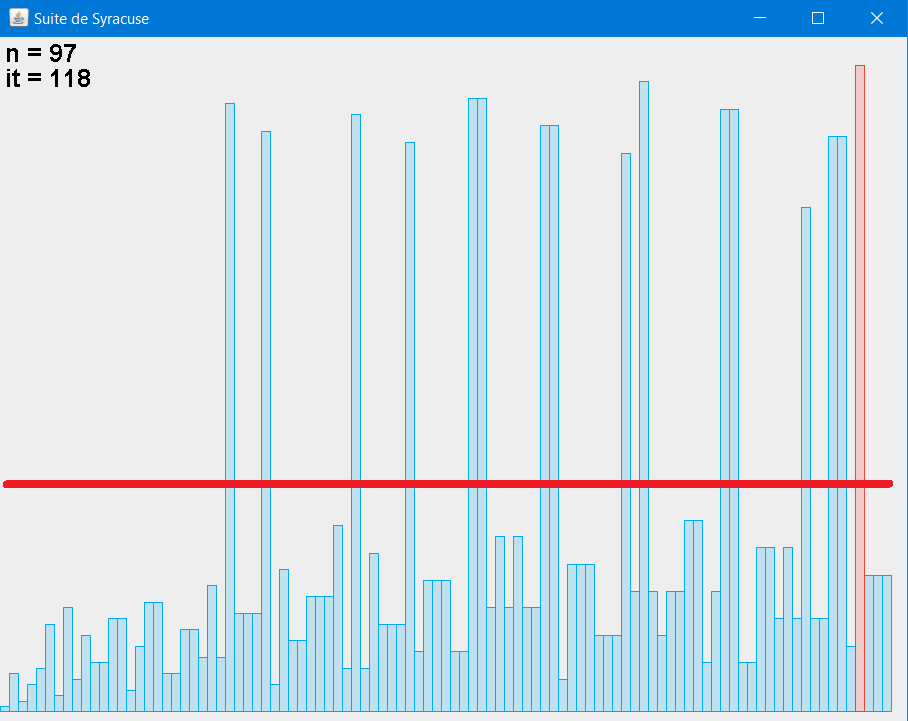
\includegraphics[scale=0.5]{images/syracuse_pics.PNG}
\end{center}
\end{frame}

\begin{frame}
Exemples de nombres qui ne sont pas des pics :
\begin{center}
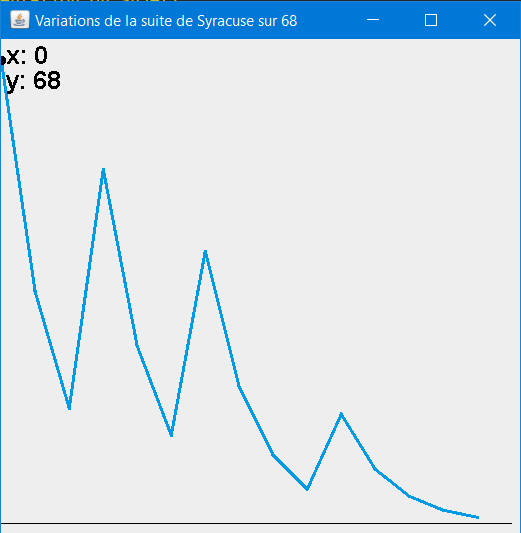
\includegraphics[scale=0.45]{images/syracuse_var_68.PNG}
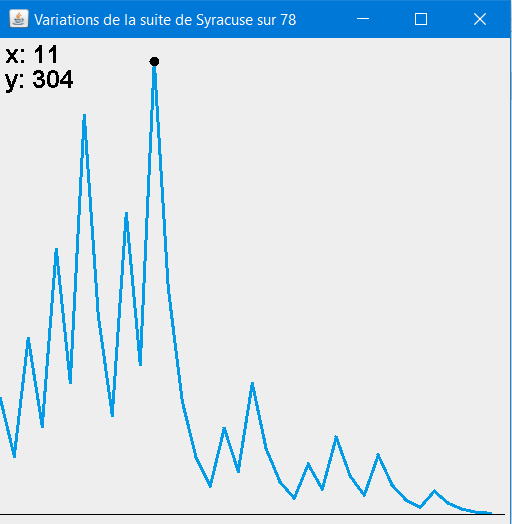
\includegraphics[scale=0.46]{images/syracuse_var_78.PNG}
\end{center}
\end{frame}

\subsection{Test avec 5n+1}
\begin{frame}
Problèmes pour utiliser nos graphiques avec 5n+1 :
\begin{itemize}
\item Présence de cycles
\item Pour n=5 : 26, 13, 66, 33, 166, 83, 416, 208, 104, 52, 26, 13, etc...
\item Pour n=13 : 66, 33, 166, 83, 416, 208, 104, 52, 26, 13, etc...
\item Pour n=7 on a une divergence
\end{itemize}
\end{frame}

\section*{}
\subsection*{Réalisation des objectifs}
\begin{frame}
\begin{itemize}
\item Crible d'Eratosthène
\item Petit théorème de Fermat
\item Exponentiation modulaire
\item Spirale d'Ulam
\item Suite de Syracuse
\item Nombres de Mersenne
\item Interpolation Lagrangienne
\end{itemize}
\end{frame}

\subsection*{Améliorations possibles}
\begin{frame}
\begin{itemize}
\item Liste chaînée pour le crible d'Eratosthène
\item Optimisé la recherche la recherche de nombres à partir d'un fichier
\item Amélioration de la façon de trouver des polynômes générateurs
\end{itemize}
\end{frame}

\end{document}
